\chapter{Impostazione di seL4}
Come primo approccio per arrivare alla scrittura di questa tesi ho innanzitutto fatto una ricerca sulla letteratura che si trova disponibile riguardo a seL4, nonostante sia poca e principalmente fornita da Trustworthy (TS) stesso è comunque sufficiente per avere una conoscenza abbastanza approfondita del microkernel.\\
SeL4 è un sistema open-source dunque lo step successivo è stato quello di scaricare seL4 e sperimentare con mano le funzionalità, ovviamente questo ha richiesto un approfondimento più tecnico e specifico, rispetto a quanto fatto finora, di alcuni aspetti come la gestione della memoria fisica e virtuale, l'IPC ecc. che verranno trattati in questo capitolo.

\section{Prerequisiti}
Come prima cosa ho installato sul mio portatile VirtualBox in quanto come consigliato dalle guide fornite da TS sarebbe ottimale lavorare in ambiente Linux, non avendo una partizione del portatile con Linux ho inizialmente pensato di utilizzare una macchina virtuale così da lasciare inalterato il mio computer e comunque avere a disposizione un sistema operativo Linux su cui lavorare. Andando avanti con il set-up del sistema per iniziare a lavorare su seL4 però ho incontrato una prima difficoltà: lo spazio, purtroppo lo spazio nel portatile non era tantissimo, la macchina virtuale, considerando il sistema operativo e l'installazione dei vari prerequisiti per poter far girare il microkernel, cominciava ad occupare una quantità non trascurabile di GB, dunque ho dovuto cercare un'alternativa; Per sopperire al problema mi sono procurato un SSD su cui sono andato a copiare la partizione creata in VirtualBox continuando la sperimentazione sul microkernel lavorando sull'SSD esterno collegato via USB.\\
Per lavorare su seL4 è necessario avere installato sul sistema dei programmi che simulino un'architettura su cui farlo girare, per fare ciò è necessario installare delle dipendenze (prerequisiti) cioè compilatori, emulatori software vari e librerie affinché sia possibile utilizzare seL4.\\
Prima di tutto ho installato Google repo, così da poter clonare i repository git:
\definecolor{codegreen}{rgb}{0,0.6,0}
\definecolor{codegray}{rgb}{0.5,0.5,0.5}
\definecolor{codepurple}{rgb}{0.58,0,0.82}
\definecolor{backcolour}{rgb}{0.95,0.95,0.92}
\lstdefinestyle{mystyle}{
    backgroundcolor=\color{backcolour},   
    commentstyle=\color{codegreen},
    keywordstyle=\color{magenta},
    numberstyle=\tiny\color{codegray},
    stringstyle=\color{codepurple},
    basicstyle=\ttfamily\footnotesize,
    breakatwhitespace=false,         
    breaklines=true,                 
    captionpos=b,                    
    keepspaces=true,                  
    numbersep=5pt,                  
    showspaces=false,                
    showstringspaces=false,
    showtabs=false,                  
    tabsize=2
}

\lstset{style=mystyle}

\begin{lstlisting}[language=bash]
sudo apt-get install repo
\end{lstlisting}
build-essential, cmake, ninja, curl, python e QEMU abbreviazione di Quick EMUlator, un emulatore open-source che permette di emulare un'architettura informatica e che permette di simulare diversi sistemi operativi, in questo caso è fondamentale perchè permette l'esecuzione di seL4:
\begin{lstlisting}[language=bash]
sudo apt-get install build-essential
sudo apt-get install cmake ccache ninja-build cmake-curses-gui
sudo apt-get install libxml2-utils ncurses-dev
sudo apt-get install curl git doxygen device-tree-compiler
sudo apt-get install u-boot-tools
sudo apt-get install python3-dev python3-pip python-is-python3
sudo apt-get install protobuf-compiler python3-protobuf
sudo apt-get install qemu-system-arm qemu-system-x86 qemu-system-misc
pip3 install --user setuptools
pip3 install --user sel4-deps
\end{lstlisting}
Altro componente fondamentale è CAmkES (component architecture for microkernel-based embedded systems), un framework per realizzare velocemente sistemi multiserver affidabili basati su microkernel:
\begin{lstlisting}[language=bash]
pip3 install --user camkes-deps
curl -sSL https://get.haskellstack.org/ | sh
sudo apt-get install haskell-stack
sudo apt-get install clang gdb
sudo apt-get install libssl-dev libclang-dev libcunit1-dev libsqlite3-dev
sudo apt-get install qemu-kvm
\end{lstlisting}
Dopodiché sono passato alle dipendenze per l'installazione di Isabelle (theorem prover) che serve per la verifica automatica di sistemi software e hardware:
\begin{lstlisting}[language=bash]
sudo apt-get install \
    python3 python3-pip python3-dev \
    gcc-arm-none-eabi build-essential libxml2-utils ccache \
    ncurses-dev librsvg2-bin device-tree-compiler cmake \
    ninja-build curl zlib1g-dev texlive-fonts-recommended \
    texlive-latex-extra texlive-metapost texlive-bibtex-extra \
    mlton-compiler haskell-stack repo
\end{lstlisting}
Ancora dipendenze Python e Haskell
\begin{lstlisting}[language=bash]
pip3 install --user --upgrade pip
pip3 install --user sel4-deps

stack upgrade --binary-only
which stack # should be $HOME/.local/bin/stack
stack install cabal-install
\end{lstlisting}
Con questa serie di comandi bash il sistema operativo Linux, per la precisione Ubuntu 22.04.2 LTS, ha tutti i prerequisiti necessari per procedere alla configurazione.

\section{Configurazione}
Lo step successivo è stato quello di recuperare, attraverso repo, la collezione di repository necessari per la verifica di seL4; in particolare contiene il sorgente del kernel, il theorem prover Isabelle/HOL e HOL4 e lo strumento di verifica binaria.
\begin{lstlisting}[language=bash]
mkdir verification
cd verification
repo init -u https://git@github.com/seL4/verification-manifest.git
repo sync
\end{lstlisting}
A questo punto  si avrà quindi una cartella con questa struttura:
\dirtree{%
.1 verification.
.2 HOL4/.
.2 graph-refine/.
.2 isabelle/.
.2 l4v/.
.2 seL4/.
}
Il che indica che l'importazione delle repository è andata a buon fine, quindi possiamo procedere alla configurazione di Isabelle posizionandosi nella cartella \texttt{l4v}:
\begin{lstlisting}[language=bash]
mkdir -p ~/.isabelle/etc
cp -i misc/etc/settings ~/.isabelle/etc/settings
./isabelle/bin/isabelle components -a
./isabelle/bin/isabelle jedit -bf
./isabelle/bin/isabelle build -bv HOL
\end{lstlisting}
Questa serie di comandi bash daranno come risultato:
\begin{itemize}
	\item la creazione di una cartella per le impostazioni utente di Isabelle.
	\item installazione delle impostazione Isabelle per L4.verified \cite{l4v} il quale è una repository che contiene formalismi per la verifica di seL4.
	\item download di Scala, Java JDK, PolyML ed altri dimostratori (prover) esterni.
	\item compilazione del Prover IDE (PIDE) jEdit di Isabelle
\end{itemize} 

\section{Avvio di SeL4}
Terminata la prima fase di installazione dei prerequisiti e di configurazione mi sono procurato ciò che servirà poi per eseguire i test delle varie funzionalità di seL4:
\begin{lstlisting}[language=bash]
mkdir seL4test
cd seL4test
repo init -u https://github.com/seL4/sel4test-manifest.git
repo sync
\end{lstlisting}
Con questi comandi si va a creare una directory \texttt{seL4test} al cui interno ci saranno tutte le direttive e le librerie necessarie per eseguire i vari test e scaricare anche il kernel stesso, attraverso il comando \texttt{repo}.\\
Dopodichè è stato necessario creare una cartella \texttt{build-x86} di configurazine per QEMU in modo da indicargli il target su cui eseguire le simulazioni:
\begin{lstlisting}[language=bash]
mkdir build-x86
cd build-x86
../init-build.sh -DPLATFORM=x86_64 -DSIMULATION=TRUE
ninja
\end{lstlisting}
Il comando \texttt{ninja}, che si vedrà spesso a seguire, è un assembler che permette di fare il build di sistemi anche complessi molto velocemente.\\
A questo punto è possibile eseguire il comando \texttt{./simulate} che farà partire la simulazione e dopo una lunga serie di test (IPC, chiamate di sistema, thread...) che appariranno nel terminale, concluderà, se tutto è andato a buon fine, con:\\
\texttt{All is well in the universe}\\
Il che indica che seL4 può essere utilizzato in questo ambiente simulato.
\begin{figure}[H]
  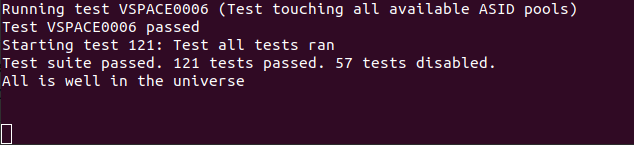
\includegraphics[width=\linewidth]{img/PrimaSimulazione.png}
  \label{fig:Prima simulazione}
\end{figure}

\section{Programmazione con le API livello kernel di seL4}
Una volta che mi sono procurato tutti i prerequisiti necessari e appurato che seL4 può girare senza problemi ho iniziato a prendere familiarità con il sistema seguendo dei tutorial forniti dalla seL4 Foundation che sono programmi semicompleti creati appositamente per sperimentare e far comprendere le funzionalità del sistema, in particolare con le API di seL4. \cite{sel4API}\\
Come ormai già visto più volte sopra ho recuperato l'ambiente per eseguire i tutorial attraverso l'uso di \texttt{repo}:
\begin{lstlisting}[language=bash]
mkdir sel4-tutorials-manifest
cd sel4-tutorials-manifest
repo init -u https://github.com/seL4/sel4-tutorials-manifest
repo sync
\end{lstlisting}
Ogni tutorial ha una sua repository da importare nell'ambiente di lavoro nella quale, tra gli altri file e cartelle, c'è (solitamente) un main.c che sarà quello su cui andare a fare le modifiche per completare il tutorial.

\subsection{Capability}
Prima di tutti ho fatto un approfondimento sulle capability:\\
Come già detto nel capitolo precedente una capability è un token unico che dà accesso ad un'entità del sistema, un puntatore con dei diritti di accesso. In seL4 ci sono 3 tipi di capability:
\begin{enumerate}
	\item capability che controllano l'accesso ad entità del kernel come i thread control block (TCB)
	\item capability che controllano l'accesso a risorse astratte tipo gli interrupt 
	\item untyped capability che sono responsabili per la gestione della memoria
\end{enumerate}
Tutte le capability delle risorse del kernel sono date dal processo root all'inizializzazione del sistema, un pò come il processo \texttt{init} nei sistemi unix che è padre di tutti i processi. Quando parliamo di capability ci sono 3 termini fondamentali CNode, CSlot e CSpace:
il primo di questi è l'abbreviazione di capability-node ed è un oggetto che contiene delle capability, possiamo pensarlo come un vettore (array) di capability, questi elementi dell'array sono chiamati CSlot (capability-slot) ed ogni CSlot può avere due stati: \texttt{empty} o \texttt{full}, ciò equivale che il CNode ha, rispettivamente, una capability nulla oppure una capability ad una risorsa del kernel, per convenzione il primo CSlot quindi quello situato alla posizione 0 del vettore è nullo. Invece un CSpace (capability-space) è il range completo di capability accessibili da un thread che può essere composto da uno o più CNode.
Per fare riferimento ad una capability ed eseguire operazioni su di essa è necessario fare un \texttt{adress} (indirizzamento) della capability, per farlo ci sono due modi per in seL4: tramite \textit{invocazione} o con \textit{indirizzamento diretto}.\\
Invocazione: ogni thread ha uno speciale CNode installato nel suo TCB noto come \texttt{CSpace root}, questo può essere nullo, ad esempio quando il thread non è autorizzato a invocare nessuna capability, o può avere una capability ad un certo CNode. Quando si vuole fare un addressing di una capability attraverso invocazione un CSlot viene indirizzato implicitamente invocando il CSpace root del thread che sta facendo l'invocazione.\\
Indirizzamento diretto: questo metodo permette di specificare il CNode piuttosto che utilizzare implicitamente il CSpace root, questo tipo di addressing  è usato principalmente per costruire e manipolare i CSpace, potenzialmente il CSpace di un altro thread.\\
L'esercizio proposto in questa sezione è un programma in linguaggio C con una serie di errori da risolvere, il primo tra questi è un errore nel settaggio del numero di byte del CNode:
\begin{lstlisting}[language=C++]
int main(int argc, char *argv[]) {

    /* parse the location of the seL4_BootInfo data structure from
    the environment variables set up by the default crt0.S */
    seL4_BootInfo *info = platsupport_get_bootinfo();

    size_t initial_cnode_object_size = BIT(info->initThreadCNodeSizeBits);
    printf("Initial CNode is %zu slots in size\n", initial_cnode_object_size);
    size_t initial_cnode_object_size_bytes = 0; // TODO
    printf("The CNode is %zu bytes in size\n", 	initial_cnode_object_size_bytes);
\end{lstlisting}
Chiaramente \texttt{initial\_cnode\_object\_size\_bytes} non può essere 0, il suo valore invece sarà dato dal numero degli slot del CNode moltiplicato per le dimensione in bit di ognuno di essi $\rightarrow$ \texttt{initial\_cnode\_object\_size * (1u << seL4\_SlotBits)}.\\
Eseguendo nuovamente il codice questo darà un errore: \texttt{Attempted to invoke a null cap} questo accade perchè il codice cerca di impostare la priorità del TCB del thread invocando l'ultimo CSlot del CSpace che è vuoto
\begin{lstlisting}[language=C++]
seL4_CPtr first_free_slot = info->empty.start;
seL4_Error error = seL4_CNode_Copy(seL4_CapInitThreadCNode, first_free_slot, seL4_WordBits, seL4_CapInitThreadCNode, seL4_CapInitThreadTCB, seL4_WordBits, seL4_AllRights);
ZF_LOGF_IF(error, "Failed to copy cap!");
%seL4_CPtr last_slot = info->empty.end - 1;
// TODO

/* set the priority of the root task */
error = seL4_TCB_SetPriority(last_slot, last_slot, 10);
ZF_LOGF_IF(error, "Failed to set priority");
\end{lstlisting}
Dunque per risolvere il problema è necessario fare un'altra copia della capability del TCB dentro l'ultimo slot del CNode: per fare ciò utilizziamo \texttt{seL4\_CNode\_Copy} che prende come parametri (destination root, slot, depth, source root, slot, depth, rights) dove depth indica quanto bisogna attraversare il CNode per arrivare al CSlot e rights sono i diritti ereditati dalla nuova capability:
\begin{lstlisting}[language=C++]
seL4_CNode_Copy(seL4_CapInitThreadCNode, last_slot, seL4_WordBits, seL4_CapInitThreadCNode, first_free_slot, seL4_WordBits, seL4_AllRights);
\end{lstlisting}
Dove \texttt{first\_free\_slot} è lo slot in cui è stata fatta una copia della capability del TCB del thread iniziale qualche riga di codice sopra.\\
Rieseguendo il programma non viene più mostrato l'errore predente ma c'è comunque un altro errore: \texttt{first\_free\_slot is not empty} questo avviene perchè il codice cerca di spostare \texttt{first\_free\_slot} e \texttt{last\_slot} in se stessi, questo non è possibile (perchè è già presente una capability, cioè se stessa) ed è in realtà un escamotage per controllare se un CSlot è vuoto.
\begin{lstlisting}[language=C++]
// TODO 
         
// check first_free_slot is empty
error = seL4_CNode_Move(seL4_CapInitThreadCNode, first_free_slot, seL4_WordBits, seL4_CapInitThreadCNode, first_free_slot, seL4_WordBits);
ZF_LOGF_IF(error != seL4_FailedLookup, "first_free_slot is not empty");

// check last_slot is empty
error = seL4_CNode_Move(seL4_CapInitThreadCNode, last_slot, seL4_WordBits, seL4_CapInitThreadCNode, last_slot, seL4_WordBits);
ZF_LOGF_IF(error != seL4_FailedLookup, "last_slot is not empty");
\end{lstlisting}
Quindi per risolvere il problema è necessario eliminare le due capability, questo può essere fatto in due modi: eliminando le due copie delle capability usando \texttt{seL4\_CNode\_Delete} oppure con \texttt{seL4\_CNode\_Revoke} sulla capability originale da cui sono state fatte le copie, quest'ultima API elimina tutte le capability figlie di essa. Per fare più velocemente ho utilizzato il secondo metodo che richiede come parametri il CNode e la posizione dentro di esso in cui andare a recuperare la capability (CNode, index, depth):
\begin{lstlisting}[language=C++]
seL4_CNode_Revoke(seL4_CapInitThreadCNode, seL4_CapInitThreadTCB, seL4_WordBits);
\end{lstlisting}
L'esercitazione conclude con la sospensione del thread corrente: \footnote{codice completo \cite{capability}}
\begin{lstlisting}[language=C++]
seL4_TCB_Suspend(seL4_CapInitThreadTCB);
\end{lstlisting}

\subsection{Gestione delle memoria}
Nella sezione precedente quando ho elencato i tipi di capability presenti in seL4 come terza ho elencato le \texttt{untyped capability}, queste sono il modo con il quale è possibile gestire la memoria fisica nel microkernel seL4.\\
Ad accezione di una piccola parte di memoria del kernel tutta la restante è gestita a livello utente, le capability a tutta la memoria fisica disponibile vengono passate al processo root come capability alla \texttt{untyped memory}, non altro è che un blocco contiguo di memoria fisica con una dimensione ben specifica, di conseguenza avremo le \texttt{untyped capability} che sono capability alla \texttt{untyped memory}. Inoltre le untyped capability possono essere riscritte in oggetti del kernel insieme alla capability oppure in ulteriori untyped capability più piccole.\\
Le untyped capability hanno anche un flag booleano \texttt{device} che inidca se la memoria è scrivibile dal kernel oppure no: può essere in un area non accessibile dal kernel o riservata ad altri dispositivi.\\
Invocazione: esiste un unico modo per invocare una untyped capability in seL4 cioè attraverso l'utilizzo dell'API \texttt{seL4\_Untyped\_Retype} che serve per creare una nuova capability da una untyped capability: nello specifico, questo retype darà accesso a un sottoinsieme della memoria della capability di origine che può essere una untyped capability più piccola o può puntare ad un nuovo oggetto con un tipo specifico.
\begin{lstlisting}[language=C++]
seL4_Untyped_Retype(parent_untyped, // the untyped capability to retype
                    seL4_UntypedObject, // type
                    untyped_size_bits,  //size
                    seL4_CapInitThreadCNode, // root
                    0, // node_index
                    0, // node_depth
                    child_untyped, // node_offset
                    1); // num_caps
\end{lstlisting}
Le untyped capability sono ritipate in maniera incrementale seguendo una politica greedy a partire dall'untyped invocato, ogni untyped capability mantiene un singolo watermark, con gli indirizzi prima di esso non disponibili e quelli successivi liberi, la memoria non può essere liberata fino a che tutti i figli non vengono revocati, dove i figli non altro sono che le nuove capability che vengono create da una untyped capability.\\
Come per la sezione sopra anche qui c'è una repository da scaricare con all'interno un file main.c, che una volta compilato e avviato, stampa a video una lista di tutte le untyped capability fornite dal processo root all'avvio; alla fine di questa segnala un errore \texttt{Untyped Retype: Requested UntypedItem size too small.} e ciò succede perchè il programma sta tentando di creare una untyped di dimensione 0:
\begin{lstlisting}[basicstyle=\tiny, language=C++]
int main(int argc, char *argv[]) {
    /* parse the location of the seL4_BootInfo data structure from
    the environment variables set up by the default crt0.S */
    seL4_BootInfo *info = platsupport_get_bootinfo();


    printf("    CSlot   \tPaddr           \tSize\tType\n");
    for (seL4_CPtr slot = info->untyped.start; slot != info->untyped.end; slot++) {
        seL4_UntypedDesc *desc = &info->untypedList[slot - info->untyped.start];
        printf("%8p\t%16p\t2^%d\t%s\n", (void *) slot, (void *) desc->paddr, desc->sizeBits, desc->isDevice ? "device untyped" : "untyped");
    }
    seL4_Error error;

    // list of general seL4 objects
    seL4_Word objects[] = {seL4_TCBObject, seL4_EndpointObject, seL4_NotificationObject};
    // list of general seL4 object size_bits
    seL4_Word sizes[] = {seL4_TCBBits, seL4_EndpointBits, seL4_NotificationBits};
    
    // TODO
    seL4_Word untyped_size_bits = 0; //ERRORE GENERATO QUI
    seL4_CPtr parent_untyped = 0;
    seL4_CPtr child_untyped = info->empty.start;

    // First, find an untyped big enough to fit all of our objects
    for (int i = 0; i < (info->untyped.end - info->untyped.start); i++) {
        if (info->untypedList[i].sizeBits >= untyped_size_bits && !info->untypedList[i].isDevice) {
            parent_untyped = info->untyped.start + i;
            break;
        }
    }
\end{lstlisting}
Per risolvere questo problema è necessario assegnare una dimensione consona alla variabile \texttt{untyped\_size\_bits}: dato che poi dobbiamo cercare uno spazio per tutti gli elementi di \texttt{objects[]} e considerato che la somma di \texttt{seL4\_EndpointBits} e \texttt{seL4\_NotificationBits} è inferiore a \texttt{seL4\_TCBBits} possiamo attribuire alla variabile: \texttt{seL4\_TCBBits + 1}, in quanto essendo in bit quel +1 fa raddoppiare il numero di byte visto che lo spazio sarà $ 2^{seL4\_TCBBits + 1} $ bit che sono sufficienti per contenere tutti e tre gli elementi\\
Eseguendo di nuovo il programma questo procederà fino a che non segnalerà un ulteriore errore \texttt{Failed to set priority}
\begin{lstlisting}[language=C++]
// create an untyped big enough to retype all of the above objects from
error = seL4_Untyped_Retype(parent_untyped, seL4_UntypedObject, untyped_size_bits, seL4_CapInitThreadCNode, 0, 0, child_untyped, 1);
ZF_LOGF_IF(error != seL4_NoError, "Failed to retype");

// use the slot after child_untyped for the new TCB cap:
seL4_CPtr child_tcb = child_untyped + 1;
// TODO

// try to set the TCB priority
error = seL4_TCB_SetPriority(child_tcb, seL4_CapInitThreadTCB, 10);
ZF_LOGF_IF(error != seL4_NoError, "Failed to set priority");
\end{lstlisting}
L'errore viene generato perchè \texttt{child\_tcb} è un CSlot vuoto, per risolvere è sufficiente assegnare al CSlot una capability creando un TCB object da \texttt{child\_untyped}
\begin{lstlisting}[language=C++]
seL4_Untyped_Retype(child_untyped, seL4_TCBObject, 0, seL4_CapInitThreadCNode, 0, 0, child_tcb, 1);
\end{lstlisting}
Con questa linea di codice il problema viene risolto ma l'esecuzione viene stoppata da un altro errore \texttt{Endpoint cap is null cap}
\begin{lstlisting}[language=C++]
// use the slot after child_tcb for the new endpoint cap:
seL4_CPtr child_ep = child_tcb + 1;
// TODO

// identify the type of child_ep
uint32_t cap_id = seL4_DebugCapIdentify(child_ep);
ZF_LOGF_IF(cap_id == 0, "Endpoint cap is null cap");
\end{lstlisting}
Questo errore è molto simile al precedente si sta cercando di identificare un endpoint nullo, quindi per risolvere il problema è necessario creare un endpoint object sempre da \texttt{child\_untyped} e mettere la capability nel CSlot \texttt{child\_ep}
\begin{lstlisting}[language=C++]
seL4_Untyped_Retype(child_untyped, seL4_EndpointObject, 0, seL4_CapInitThreadCNode, 0, 0, child_ep, 1);
\end{lstlisting}
Alla fine il programma tenta di allocare tutto il \texttt{child\_untyped} come endpoint ma fallisce perchè tutto lo spazio è stato consumato dalla allocazioni fatte precedentemente, quindi la soluzione è fare una \texttt{seL4\_CNode\_Revoke} (vista sopra) su di esso in modo che tutto le spazio venga liberato e così facendo il programma termina con successo. \footnote{codice completo \cite{untyped}}
\begin{lstlisting}[language=C++]
// revoke the child untyped
error = seL4_CNode_Revoke(seL4_CapInitThreadCNode, child_untyped, seL4_WordBits);

// allocate the whole child_untyped as endpoints
// Remember the sizes are exponents, so this computes 2^untyped_size_bits / 2^seL4_EndpointBits:
seL4_Word num_eps = BIT(untyped_size_bits - seL4_EndpointBits);
error = seL4_Untyped_Retype(child_untyped, seL4_EndpointObject, 0, seL4_CapInitThreadCNode, 0, 0, child_tcb, num_eps);
ZF_LOGF_IF(error != seL4_NoError, "Failed to create endpoints.");

printf("Success\n");
\end{lstlisting}

\subsection{Virtual memory management}
Incipit: cos'è la memoria virtuale: "la memoria virtuale è un'architettura di sistema capace di simulare uno spazio di memoria centrale (memoria primaria) maggiore di quello fisicamente presente o disponibile, dando l'illusione all'utente di un enorme quantitativo di memoria". \cite{MemoriaVirtuale} Questa tecnica porta con sè diversi vantaggi, uno tra questi la sicurezza dovuta all'isolamento della memoria, la possibilità di condivisione di alcune pagine di memoria tra più processi (tipo quelle contenenti le librerie che ovviamente non cambiano e quindi possono essere usate in contemporanea da più processi) e infine l'ultimo ma allo stesso tempo il principale vantaggio: avere a disposizione molta più memoria centrale di quella che in realtà è disponibile. Giustamente viene da chiedersi com'è possibile tutto ciò e il meccanismo alla base è quello di utilizzare una memoria ausiliaria, solitamente la memoria di massa, per allocare una certa parte di memoria che non è stata utilizzata recentemente; nel momento in cui viene richiesto nuovamente la porzione di dati salvati nella memoria ausiliaria (oppure si libera spazio nella memoria centrale) i dati relativi vengono prelevati e copiati nuovamente in memoria centrale, questo processo che prende il nome di \textit{swapping}. In presenza di memoria virtuale quindi vengono mappati gli indirizzi di memoria in indirizzi \textit{fisici} e \texttt{logici}, i programmi lavoreranno solo con indirizzi logici (quindi viene anche facilitata la programmazione) e poi a livello di CPU avverrà un processo di traduzione negli indirizzi fisici.\\
SeL4 non fornisce strumenti per la gestione della memoria virtuale al di là delle primitive per gestione dell'hardware, quindi il servizio di mappatura della memoria e lo swapping deve essere gestito a livello utente che ha tutta la libertà di gestirlo in base alle esigenze del sistema. SeL4 mette dunque a disposizione degli oggetti appositi chiamati \textit{VSpace} (virtual address space), simili ai CSpace, e sono composti da oggetti forniti dal kernel che variano in base all'architettura hardware (x86\_64, RISC-V, ARM).\\
Per mappare le pagine sono necessari degli "intermediate hardware virtual memory objects", praticamente per mappare una pagina è necessario creare una struttura intermedia che varia in base all'architettura: ad esempio nei sistemi x86\_64 per mappare una pagina sono necessari questi 3 oggetti \texttt{seL4\_PDPT, seL4\_PageDirectory, seL4\_PageTable}. Le API di seL4 forniscono varie funzioni per la mappatura delle memoria in base all'architettura in cui sta girando seL4, tutte le funzione di mapping prendono 3 argomenti principali:
\begin{itemize}
	\item il VSpace in cui mappare l'oggetto
	\item l'indirizzo virtuale su cui mappare l'oggetto
	\item attributi della memoria virtuale che dipendono dall'architettura 
\end{itemize}
Esempio di mappatura di un oggetto \texttt{seL4\_PDPT} ad un certo indirizzo \texttt{TEST\_VADDR}:
\begin{lstlisting}[language=C++]
seL4_X86_PDPT_Map(pdpt, seL4_CapInitThreadVSpace, TEST_VADDR, seL4_X86_Default_VMAttributes);
\end{lstlisting}
Una volta che le strutture di paginazione intermedie sono state mappate in un certo range di indirizzi virtuali, i frame fisici possono essere mappati in quel range attraverso l'invocazione del frame capability.\\
Esempio di mappatura di un frame:
\begin{lstlisting}[language=C++]
seL4_X86_Page_Map(frame, seL4_CapInitThreadVSpace, TEST_VADDR, seL4_CanRead, seL4_X86_Default_VMAttributes);
\end{lstlisting}
Come si vede questo metodo prende un argomento in più perchè per mappare i frame vengono richiesti anche i diritti che determineranno il tipo di mappatura(nell'esempio sopra diritti di sola lettura).\\
Il tutorial di questa sezione fornisce un programma che all'avvio termina lanciando l'errore \texttt{Missing intermediate paging structure at level 30} 
\begin{lstlisting}[language=C++]
int main(int argc, char *argv[]) {
    /* parse the location of the seL4_BootInfo data structure from
    the environment variables set up by the default crt0.S */
    seL4_BootInfo *info = platsupport_get_bootinfo();
    seL4_Error error;
    seL4_CPtr frame = alloc_object(info, seL4_X86_4K, 0);
    seL4_CPtr pdpt = alloc_object(info, seL4_X86_PDPTObject, 0);
    seL4_CPtr pd = alloc_object(info, seL4_X86_PageDirectoryObject, 0);
    seL4_CPtr pt = alloc_object(info, seL4_X86_PageTableObject, 0);

	// TODO
	
	// TODO

    /* map a PDPT at TEST_VADDR */
    error = seL4_X86_PDPT_Map(pdpt, seL4_CapInitThreadVSpace, TEST_VADDR, seL4_X86_Default_VMAttributes);

    /* map a read-only page at TEST_VADDR */
    error = seL4_X86_Page_Map(frame, seL4_CapInitThreadVSpace, TEST_VADDR, seL4_CanRead, seL4_X86_Default_VMAttributes);
    if (error == seL4_FailedLookup) {
        printf("Missing intermediate paging structure at level %lu\n", seL4_MappingFailedLookupLevel());
    }
    ZF_LOGF_IF(error != seL4_NoError, "Failed to map page");
\end{lstlisting}
Errore dovuto al fatto che per mappare una pagina tutte le strutture di paginazione intermedie devono essere mappate; il valore \texttt{30} equivale alla costante \texttt{SEL4\_MAPPING\_LOOKUP\_NO\_PD} il che ci indica che è necessario mappare un oggetto page directory che può essere fatto con l'apposito metodo \texttt{seL4\_X86\_PageDirectory\_Map}:
\begin{lstlisting}[language=C++]
seL4_X86_PageDirectory_Map(pd, seL4_CapInitThreadVSpace, TEST_VADDR, seL4_X86_Default_VMAttributes);
\end{lstlisting}
Ricompilando ed eseguendo il codice appare un errore simile al precedente \texttt{Missing intermediate paging structure at level 21} dove il valore \texttt{21} questa volta indica la costante \texttt{SEL4\_MAPPING\_LOOKUP\_NO\_PT} che suggerisce di mappare un oggetto page table:
\begin{lstlisting}[language=C++]
seL4_X86_PageTable_Map(pt, seL4_CapInitThreadVSpace, TEST_VADDR, seL4_X86_Default_VMAttributes);
\end{lstlisting}
Adesso il codice procede mappando la pagina però successivamente (come si può leggere nel codice sotto) avviene un tentativo di scrittura sulla pagina che genera un errore perchè la pagina era stata mappata in sola lettura \texttt{seL4\_CanRead}, l'errore può dunque essere aggiustato facendo una rimappatura della pagina questa volta in lettura e scrittura:\footnote{codice completo \cite{mapping}}
\begin{lstlisting}[language=C++]
seL4_X86_Page_Map(frame, seL4_CapInitThreadVSpace, TEST_VADDR, seL4_ReadWrite, seL4_X86_Default_VMAttributes);
\end{lstlisting}
Ovviamente le pagine possono anche essere "unmappate" utilizzando \texttt{unmap} sulla pagina o su qualsiasi struttura intermedia di paginazione oppure eliminando la capability finale di qualsiasi struttura di paginazione.

\subsection{Thread}
SeL4 per rappresentare l'esecuzione di un processo e gestire i tempi di esecuzione fornisce i thread, essi sono realizzati attraverso \textit{thread control block object} (TCBs) e ce ne sono uno per ogni thread del kernel.\\
Come sappiamo in un SO è lo scheduler a decidere quale processo e per quanto tempo può utilizzare la CPU, in seL4, come avevamo già visto nel capitolo precedente, la politica di scheduling è un integrazione di round-robin e scheduling sulla priorità: lo scheduler sceglie i thread con maggiore priorità che sono pronti e se ci sono processi con la stessa priorità questi saranno scelti in ordine FIFO seconda la politica round-robin. La priorità è determinata da un range che va da 0 (\texttt{seL4\_MinPrio}) a 255 (\texttt{seL4\_MaxPrio}), oltre alla priorità un TCBs contiene anche un \textit{maximum control priority} (MCP) che serve per controllare che un processo non modifichi la priorità di un altro processo (o di se stesso) impostandola più alta della sua, quindi un processo che vuole modificare una priorità deve fornire la sua capability (di thread) in modo da determinare se è autorizzato a impostare quella priorità.\\
L'esercizio per questa sezione, se fatto partire senza nessuna modifica, inizialmente mostrerà a video una tabella di tutti i TCB (questo ottenuto tramite una chiamata di sistema di debug \texttt{seL4\_DebugDumpScheduler()}) e successivamente lancia un errore \texttt{Failed to retype thread: 2} come in Figura~\ref{fig:TutorialThreads}.\\
\begin{figure}[h]
  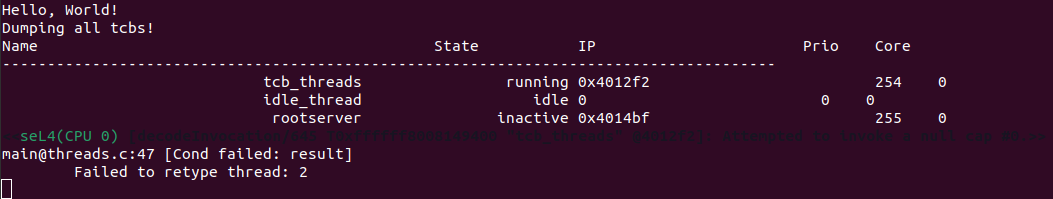
\includegraphics[width=\linewidth]{img/Threads.png}
  \caption{lista TCB}
  \label{fig:TutorialThreads}
\end{figure}
\\Questo errore avviene perchè c'è un errata invocazione del metodo: \texttt{seL4\_Untyped\_Retype()}
\begin{lstlisting}[language=C++]
// the root CNode of the current thread
extern seL4_CPtr root_cnode;
// VSpace of the current thread
extern seL4_CPtr root_vspace;
// TCB of the current thread
extern seL4_CPtr root_tcb;
// Untyped object large enough to create a new TCB object

extern seL4_CPtr tcb_untyped;
extern seL4_CPtr buf2_frame_cap;
extern const char buf2_frame[4096];

// Empty slot for the new TCB object
extern seL4_CPtr tcb_cap_slot;
// Symbol for the IPC buffer mapping in the VSpace, and capability to the mapping
extern seL4_CPtr tcb_ipc_frame;
extern const char thread_ipc_buff_sym[4096];
// Symbol for the top of a 16 * 4KiB stack mapping, and capability to the mapping
extern const char tcb_stack_base[65536];
static const uintptr_t tcb_stack_top = (const uintptr_t)&tcb_stack_base + sizeof(tcb_stack_base);

int new_thread(void *arg1, void *arg2, void *arg3) {
    printf("Hello2: arg1 %p, arg2 %p, arg3 %p\n", arg1, arg2, arg3);
    void (*func)(int) = arg1;
    func(*(int *)arg2);
    while(1);
}

int main(int c, char* arbv[]) {

    printf("Hello, World!\n");

    seL4_DebugDumpScheduler();
	// TODO
    seL4_Error result = seL4_Untyped_Retype(seL4_CapNull, seL4_TCBObject, seL4_TCBBits, seL4_CapNull, 0, 0, seL4_CapNull, 1);
    ZF_LOGF_IF(result, "Failed to retype thread: %d", result);
    seL4_DebugDumpScheduler();
\end{lstlisting}
Come si può vedere al metodo viene passato un oggetto \texttt{seL4\_CapNull} come oggetto da ritipare che ovviamente genera l'errore, dunque un modo corretto per sistemare questo errore è utilizzare gli oggetti creati nelle variabili globali del codice
\begin{lstlisting}[language=C++]
seL4_Error result = seL4_Untyped_Retype(tcb_untyped, seL4_TCBObject, seL4_TCBBits, root_cnode, 0, 0, tcb_cap_slot, 1);
\end{lstlisting}
Rieseguendo il codice vedremo che l'errore è risolto e tra la lista dei TCB adesso è presente anche quello appena creato. Dopo aver risolto questo problema se ne presenta un altro \texttt{Failed to configure thread: 2} in quanto la configurazione del TCB viene fatta tutta su valori nulli
\begin{lstlisting}[language=C++]
result = seL4_TCB_Configure(seL4_CapNull, seL4_CapNull, 0, seL4_CapNull, 0, 0, (seL4_Word) NULL, seL4_CapNull);
ZF_LOGF_IF(result, "Failed to configure thread: %d", result);
\end{lstlisting}
Il metodo \texttt{seL4\_TCB\_Configure} prende come parametri:
\begin{lstlisting}[language=C++]
seL4_Untyped_Retype(tcb, // tcb su cui operare
					fault_ep, // chi ricevera' l'IPC quando il thread fallisce
					cspace_root, // nuovo CSpace root
					cspace_root_data, // opzionale: setta il nuovo CNode
					vspace_root, // nuovo VSpace root
					vspace_root_data, // non ha effetto su x86 e ARM
					buffer, // locazione dell'IPC buffer
					bufferFrame); // IPC buffer
\end{lstlisting} 
Avendo adesso il TCB creato poco sopra è possibile configurarlo in modo da avere lo stesso CSpace e VSpace del thread corrente:
\begin{lstlisting}[language=C++]
result = seL4_TCB_Configure(tcb_cap_slot, seL4_CapNull, root_cnode, 0, root_vspace, 0, (seL4_Word) thread_ipc_buff_sym, tcb_ipc_frame);
\end{lstlisting}
Adesso l'errore che si presenta sarà un altro\\
\texttt{Failed to set the priority for the new TCB object.}\\
questo perchè la priorità data al thread ha valore 0
\begin{lstlisting}[language=C++]
result = seL4_TCB_SetPriority(tcb_cap_slot, seL4_CapNull, 0);
ZF_LOGF_IF(result, "Failed to set the priority for the new TCB object.\n");
seL4_DebugDumpScheduler();
\end{lstlisting}
Il thread corrente ha un MCP di 254 quindi è possibile assegnare questo valore come priorità, per poterlo fare è necessario anche cambiare il valore \texttt{seL4\_CapNull} e sostituirlo con il tcb del thread corrente \texttt{root\_tcb}.
Dopodiché è necessario impostare in maniera adeguata i registri iniziali in particolare il \textit{program counter} e lo \textit{stack pointer} che è possibile farlo grazie alle utility contenute in \texttt{libsel4utils}
\begin{lstlisting}[language=C++]
seL4_UserContext regs = {0};
int error = seL4_TCB_ReadRegisters(tcb_cap_slot, 0, 0, sizeof(regs)/sizeof(seL4_Word), &regs);
ZF_LOGF_IFERR(error, "Failed to read the new thread's register set.\n");

// TODO
sel4utils_set_instruction_pointer(&regs, (seL4_Word)new_thread);
// TODO
sel4utils_set_stack_pointer(&regs, tcb_stack_top);
// TODO
error = seL4_TCB_WriteRegisters(tcb_cap_slot, 0, 0, sizeof(regs)/sizeof(seL4_Word), &regs);
ZF_LOGF_IFERR(error, "Failed to write the new thread's register set.\n"
                  "\tDid you write the correct number of registers? See arg4.\n");
seL4_DebugDumpScheduler();
\end{lstlisting}
A questo punto è possibile far partire il thread ma per farlo è necessario fare un piccolo aggiustamento nel codice 
\begin{lstlisting}[language=C++]
//resume the new thread
error = seL4_TCB_Resume(seL4_CapNull);
ZF_LOGF_IFERR(error, "Failed to start new thread.\n");
while(1);
return 0;
}
\end{lstlisting}
Chiaramente il resume va fatto sul nostro \texttt{tcb\_cap\_slot} e non su \texttt{seL4\_CapNull}, ora il nuovo thread viene eseguito e mostra a video\\
\texttt{Hello2: arg1 0, arg2 0, arg3 0}\\
Come si può vedere i valori passati al nuovo thread sono tutti 0, se volessimo passare valori differente potremmo utilizzare la funzione \texttt{sel4utils\_arch\_init\_local\_context} facendo delle modifiche al codice:\footnote{codice completo \cite{threads}}
\begin{lstlisting}[language=C++]
UNUSED seL4_UserContext regs = {0};
int error = seL4_TCB_ReadRegisters(tcb_cap_slot, 0, 0, sizeof(regs)/sizeof(seL4_Word), &regs);
ZF_LOGF_IFERR(error, "Failed to read the new thread's register set.\n"
              "\tDid you write the correct number of registers? See arg4.\n");

sel4utils_arch_init_local_context((void*)new_thread,
                                  (void *)1, (void *)2, (void *)3,
                                  (void *)tcb_stack_top, &regs);
error = seL4_TCB_WriteRegisters(tcb_cap_slot, 0, 0, sizeof(regs)/sizeof(seL4_Word), &regs);
ZF_LOGF_IFERR(error, "Failed to write the new thread's register set.\n"
              "\tDid you write the correct number of registers? See arg4.\n");
\end{lstlisting}

\subsection{IPC}
InterProcess Communication è il meccanismo che utilizza il microkernel per sincronizzare lo scambio di  piccole quantità di dati e capability tra i processi. In seL4 l'IPC è facilitato dal fatto che gli ogetti del kernel sono di piccole dimensioni noti come \textit{endpoint} che fungono da porte per la comunicazione; quindi per mandare e ricevere messaggi IPC bisogna farlo attraverso invocazioni sugli endpoint.\\
I thread possono mandare messaggi sugli endpoint  con la system call \texttt{seL4\_Send} che è bloccante, mentre possono usare \texttt{seL4\_Recv} per ricevere messaggi; \texttt{seL4\_Call} invece è una chiamata di sistema che combina le due precedenti con una differenza: nella fase di ricezione il thread che usa questa funzione è bloccato su una "one-time capability" chiamata \textit{reply capability} e non sull'endpoint stesso come avverrebbe normalmente con la \texttt{seL4\_Recv}. La replay capability è contenuta nel TCB del ricevente, la system call \texttt{seL4\_Reply} invoca questa capability la quale manderà un IPC che farà risvegliare il processo bloccato. \texttt{seL4\_ReplyRecv} fa lo stesso ma invia la risposta e blocca l'endpoint fornito in una chiamata di sistema combinata.\\
Ogni thread ha un buffer che contiene il payload del messaggio IPC composto da dati e capability. Il mittente del messaggio specifica la lunghezza e il kernel copia questa quantità tra il mittente e il destinatario dell'IPC buffer. Il buffer IPC contiene  un'area limitata di \textit{message registers} (MR) che sono utilizzati per trasmettere dati sull'IPC, ogni registro ha dimensione di una parola relativo alla macchina e la lunghezza massima di un messaggio è contenuta nella costante \texttt{seL4\_MsgMaxLength}, per caricare un messaggio dentro il buffer è possibile utilizzare \texttt{seL4\_SetMR} mentre per estrarlo \texttt{seL4\_GetMR}, la quantità di parole che possono entrare in un registro è disponibile nelle costante \texttt{seL4\_FastMessageRegisters}.\\
Insieme al messaggio il kernel consegna inoltre il \textit{badge} dell'endpoint capability sul quale il mittente ha fatto l'invocazione per mandare il messaggio; gli endpoint possono essere "bedgati" usando \texttt{seL4\_CNode\_Mint} oppure \texttt{seL4\_CNode\_Mutate}, una volta che è stato messo il badge sull'endpoint questo viene trasferito a tutti i destinatari che ricevono un messaggio su quell'endpoint.\\
SeL4 usa la struttura dati \texttt{seL4\_MessageInfo\_t} per codificare la descrizione di un messaggio IPC in una singola parola (word) ed è composta dai seguenti campi:
\begin{itemize}
	\item[-] \texttt{length} la quantità di dati nel messaggio
	\item[-] \texttt{extraCaps} numero di capability nel messaggio 
	\item[-] \texttt{capsUnwrapped} marca le capability unwrapped dal kernel
	\item[-] \texttt{label} dati che verranno trasferiti che non sono statoi modificati dal kernel
\end{itemize}
Come già accennato, insieme ai dati, attraverso l'IPC, è possibile scambiare anche capability, in gergo questo viene chiamato \textit{cap transfer}:
\begin{lstlisting}[language=C++]
//Invio di una capability via IPC
seL4_MessageInfo info = seL4_MessageInfo_new(0, 0, 1, 0);
seL4_SetCap(0, free_slot);
seL4_Call(endpoint, info);

//Ricezione di una capability
seL4_SetCapReceivePath(cnode, badged_endpoint, seL4_WordBits);
seL4_Recv(endpoint, &sender);
\end{lstlisting}
Il numero di capability trasferita è codificato nella struttura dati \texttt{seL4\_MessageInfo\_t} come \texttt{extraCaps}.
Inoltre seL4 può fare la cosiddetta \textit{unwrap} (scartare) delle capability sull'IPC: se l'n-esima capability nel messaggio si riferisce all'endpoint attraverso il quale il messaggio viene inviato, la capability viene \textit{unwrapped}: il suo badge viene inserito nell'n-esima posizione dell'IPC buffer del destinatario (\texttt{caps\_or\_badges}) e il kernel setta l'n-esimo bit nel campo \texttt{capsUnwrapped} del \texttt{seL4\_MessageInfo\_t}.\\
Fastpath: avere un IPC veloce è un elemento fondamentale per i sistemi basati su microkernel in quanto tutti i servizi sono a livello utente ed essendo isolati l'unico modo per comunicare è attraverso l'IPC, dunque è necessario avere quello che si chiama \textit{fastpath}, cioè un cammino nel kernel altamente ottimizzato che garantisce velocità nell'IPC; per potersi definire tale deve soddisfare cinque condizioni:
\begin{itemize}
	\item devono essere usate le system call \texttt{seL4\_Call} o \texttt{seL4\_ReplyRecv}
	\item i dati del messaggio devono entrare nel registro \texttt{seL4\_FastMessageRegisters}
	\item i processi devono avere spazi di indirizzi validi
	\item non dovrebbero essere straferite capability 
	\item nessun altro thread nello scheduler con priorità superiore a quello sbloccato dall'IPC può essere in esecuzione
\end{itemize}
In questa sezione l'esercizio è un pò diverso, non c'è un unico file main in cui è contenuto tutto il codice ma c'è un \texttt{server.c} e due client: \texttt{client\_1.c} e \texttt{client\_2.c} i quali manderanno dei messaggi al server che farà da echo; tutti i processi hanno accesso ad un unioa endpoint capability che fornisce accesso allo stesso endpoint object.\\
Al primo avvio si ha questo output:
\begin{figure}[H]
  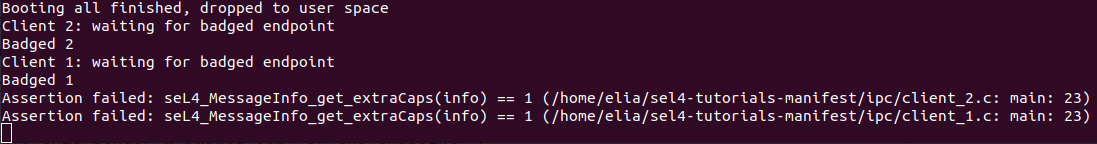
\includegraphics[width=\linewidth]{img/PrimoAvvioIPC.png}
  \label{fig:PrimoAvvio}
\end{figure}
Gli errori sono dovuti al fatto che entrambi i client si mettono in attesa sull'endpoint in attesa di un endpoint con badge tramite cap tranfer che però il server non invierà in quanto il server risponde solo ai messaggi dei client.
\begin{lstlisting}[language=C++]
// cslot containing IPC endpoint capability
extern seL4_CPtr endpoint;
// cslot containing a capability to the cnode of the server
extern seL4_CPtr cnode;
// empty cslot
extern seL4_CPtr free_slot;

int main(int c, char *argv[]) {

	seL4_Word sender;
    seL4_MessageInfo_t info = seL4_Recv(endpoint, &sender);
    while (1) {
	    seL4_Error error;
        if (sender == 0) {

             /* No badge! give this sender a badged copy of the endpoint */
             seL4_Word badge = seL4_GetMR(0);
             seL4_Error error = seL4_CNode_Mint(cnode, free_slot, seL4_WordBits,
                                                cnode, endpoint, seL4_WordBits,
                                                seL4_AllRights, badge);
             printf("Badged %lu\n", badge);

             // TODO
             
             /* reply to the sender and wait for the next message */
             seL4_Reply(info);

             /* now delete the transferred cap */
             error = seL4_CNode_Delete(cnode, free_slot, seL4_WordBits);
             assert(error == seL4_NoError);

             /* wait for the next message */
             info = seL4_Recv(endpoint, &sender);
\end{lstlisting}
Dunque per risolvere questo problema è necessario impostare il cap transfer in modo che i client ricevano l'endoint badgato:
\begin{lstlisting}[language=C++]
info = seL4_MessageInfo_new(0, 0, 1, 0);
seL4_SetCap(0, free_slot);
\end{lstlisting}
Compilando e riavviando il programma sembra vada tutto bene eccetto che il sistema si blocca
\begin{figure}[H]
  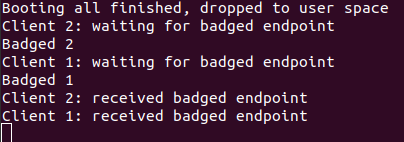
\includegraphics[width=\linewidth]{img/DopoBadgeIPC.png}
  \label{fig:AvvioDopoBedge}
\end{figure}
Questo succede perchè al server manca l'implementazione della sua funzione di echo dei messaggi che gli vengono inviati la quale può essere fatta scorrendo e stampando a video il contenuto dei message register.\\
(I client mandano rispettivamente le stringhe {"quick", "fox", "over", "lazy"} il \texttt{client\_1} mentre il \texttt{client\_2} {"the", "brown", "jumps", "the", "dog"}.)
\begin{lstlisting}[language=C++]
for (int i = 0; i < seL4_MessageInfo_get_length(info); i++) {
printf("%c", (char) seL4_GetMR(i));
}
printf("\n");
\end{lstlisting}
A questo punto però vedremo stampata a video sempre la stessa parola "the" in loop perchè il server non manda un feedback di risposta al client e di conseguenza continua a stampare l'ultima parola ricevuta.
\begin{lstlisting}[language=C++]
for (int i = 0; i < seL4_MessageInfo_get_length(info); i++) {
	printf("%c", (char) seL4_GetMR(i));
}
printf("\n");

// reply to the client and wait for the next message
info = seL4_ReplyRecv(endpoint, info , &sender);
\end{lstlisting}
A questo punto l'output sarà la stampa a video prima di tutte le parole inviate dal client 2 seguite da quelle del client 1, possiamo modificare il codice in modo da alternare le stampe dei due client utilizzando \texttt{seL4\_CNode\_SaveCaller} e \texttt{free\_slot} per salvare le risposte.
\begin{lstlisting}[language=C++]
for (int i = 0; i < seL4_MessageInfo_get_length(info); i++) {
printf("%c", (char) seL4_GetMR(i));
}
printf("\n");

error = seL4_CNode_SaveCaller(cnode, free_slot, seL4_WordBits);
assert(error == 0);
info = seL4_Recv(endpoint, &sender);
for (int i = 0; i < seL4_MessageInfo_get_length(info); i++) {
   printf("%c", (char) seL4_GetMR(i));
}
printf("\n");
seL4_Send(free_slot, seL4_MessageInfo_new(0, 0, 0, 0));

// reply to the client and wait for the next message
info = seL4_ReplyRecv(endpoint, info, &sender);
\end{lstlisting}
A questo punto l'output finale sarà il seguente:\footnote{codice completo server \cite{IPCserver}}\footnote{codice completo client\_1 \cite{IPCclient1}}\footnote{codice completo client\_2\cite{IPCclient2}}
\begin{lstlisting}[language=bash]
Client 2: received badged endpoint
the
Client 1: received badged endpoint
quick
fox
brown
jumps
over
lazy
the
dog
\end{lstlisting}
